%Tex file for Git Hub for Authors HOWTO
\documentclass[a4paper, 12pt]{article}
\usepackage{graphicx}
\title{Git and GitHub for Authors}
\author{TM Coker}
\setlength{\parskip}{1ex}
\setlength{\parindent}{0em}
%set of macros to adjust page layout
\pdfpagewidth=\paperwidth 
\pdfpageheight=\paperheight
\setlength{\marginparwidth}{20mm}
\setlength{\hoffset}{-1in}
\setlength{\voffset}{-1in}
\setlength{\textwidth}{167mm}
\setlength{\textheight}{262mm}
\setlength{\oddsidemargin}{20mm}
\setlength{\evensidemargin}{20mm}
\begin{document}
\maketitle
\section{Introduction}
\subsection{What is Git and GitHub}
Git is a software source control system, initially written by Linus Torvalds specifically to support Linux kernel development, the assessment being that other systems then available were not up to the demands of Limux development. Development of Git was started in 2005 and Git is now open--source software distributed under the GNU GPL.

In common with other systems Git provides the means for:
\begin{itemize}
\item Many programmers to collaborate on a single software application.
\item Manage releases and software version control.
\item Track changes to software as it is developed.
\item Branch a code base to allow specific issues to be worked on in parallel.
\item Merge branches back into the main code base.
\end{itemize}

Git also has a similar top level structure to other solutions -- projects or applications roughly correspond to `repositories' (often called `repos'). Within any one repo there will exist a number of branches, and typically in software development a branch represents a version of the code being developed to address one specific issue, which could be a new feature or fixing a bug. The key feature of such systems is that they maintain a full record of changes to all files that are held within the repo, for software this is required for tracking purposes, e.g. who made what change when, but it also provides a complete history of the software as it has been developed.

GitHub is effectively a cloud based implentation of Git, with a browser interface into the more sophisticated functions, such as `pull requests', code reviews, merging, release management and so on (none of which really concern authors). However GitHub cannot effectively be used on its own, it really needs a local Git implementation and as such, for our needs, Git Hub is really just cloud storage (although it does offer some facilities that your local Git application doesn't have).

\subsection{Relevance to Authors}
Authors, although they are not writing software, have similar requirements to software engineers:
\begin{itemize}
\item They develop source material in an incremental way, keeping track of changes and version information.
\item In many cases, particularly in the sciences, several authors will be collaborating on a single book, article or paper, in which case simple word processing software such as Word is limited, as is LaTex. Although alternatives such as Google Docs can be used, even these have their limits, particularly for laying out scientific papers with cross--referencing, citations and so on.
\item For authors using LaTex -- because of it's sophistication -- other than file backup software, there is no obvious solution to the need for revision control, archiving and so on.
\item Authors need to periodically archive and/or back up their material.
\item They would preferably back up to cloud storage as well as any local media -- local hard--drives, additional home file storage and so on.
\item If necessary they may want to work on two or more versions of essentially the same document, but keeping them separate.
\item They may want to retrieve an older version of the source material, either by rolling back changes or retrieving a complete set of source material that has been suitably labelled.
\end{itemize}
All these requirements are essentially the same as the ones software engineers have when writing code, although authors only need a modest subset of the full set of features that Git or any other source control system provides. However the general message is that a system like Git/GitHub has many of the features that authors look for, indeed (as we'll see below) there are setup files designed specifically for Tex/LaTex, which implies that GitHub is alreayd beng used in this way.

\textbf{Disadvantages} -- powerful though Git is, it isn't perfect, the principle limitation is that the file history isn't a simple archive of previous version of files and documents. So if you happen to want to go back a period of time to an older verison of a document, it is not as simple as browsing through folders on Windows Explorer and copy files, the \textit{only} way to get to an old version of a file is to access the storage via Git. If this is a serious concern for you, then a Git based system is not the solution for you, although other solutions such as CVS may work.

\subsection{Technical Description}
This is not in any way a full description of the inner workings of Git, but part of the purpose of this document is to explain why you might want to use Git/GitHub when you aren't already.

Unlike many equivalent systems, Git does not primarily use a client/server model, the entire system can be deployed to a single machine, although collaboration facilities would clearly be limited. In practice Git can be considered as a private file system with a set of coded utilities running on top. The utilities manage files within repos and branches, storing files, tracking changes and so on. Git has been primarily written to run on Linux and the actual user interface has always been the command line. However the system has become so successful that there are many third party applications that provide a traditional window based GUI. A little bit of web searching will quickly lead you to many examples, e.g. GitKraken, SmartGit, Fork and so on. A quick online search for `git gui' will quickly lead you to a plethora of alternatives, but be aware many are not free, or have proprietary licences or hidden drawbacks.

Notwithstanding the above, two particular implementations should be considered:
\begin{itemize}
\item Git For Windows -- this is effectively the `official' Windows version from the open--source collaboration that maintains and develops Git.
\item GitHub Desktop - assuming that you're intending to use GitHub, then GitHub Desktop seems an obvious solution for ease of integration. Open source, free and available under the MIT Licence, with reasonably good support and also a thriving community.
\end{itemize}
As a little bit of context, I'd not suggest GitHub Desktop as first choice client for actual coding. When I was last running a software team, we actually settled on Fork (which is good but not free). However for the more limited needs of authors I'd suggest that GitHub Desktop is more than adequate. As you'll see below, this is the solution that has been used by the author of this document.

\subsection{What This Document Is Not}
Although, of a necessity, this HOWTO document describes a lot of the basic features of Git and GitHub, it is not a guide to either of those systems, it is just a guide to getting set up and using those features of the system that work well for authors.

\section{Getting Setup with Git}
There are two principle steps to getting set up -- registering and creating a GitHub account, and installing your local Git application. These two can actually be done quite independently and I'd suggest you get up and running with your local Git application before setting up on Git Hub. This is particularly the case if you decide to use GitHub Desktop as this makes for a very easy process to `push' your local repos up to GitHub. The alternative workflow is to create repos on GitHub then clone them to your local machine, which works fine and is only marginally more comlex. Whichever way you end up doing it, there is a process to link your Git application to GitHub, this is fairly straightforward if you're using GitHub Desktop and is another reason to use this application.

\subsection{Assumptions}
For the rest of this guide, it is assumed that:
\begin{itemize}
\item You are running Windows 10.
\item You have chosen GitHub Desktop.
\item You are using LaTex to create your documents, MiKTex version 2.9.
\item And you are setting up GitHub Desktop before registering on GitHub.
\end{itemize}
If that is not the case, it doesn't necessarily mean that you can't use this guide, the broad steps to take should be the same regardless of actual implementation, but the screengrabs in particular may be of limited use.

\subsection{Installing and Running GitHub Desktop}
Once you've downloaded the installer run it as normal, the installation process is simple and direct and should launch the application straight away. Once its running you should see the window shown in Figure \ref{startscreen}.

\begin{figure}
\centering
\includegraphics[width=\linewidth]{startscreen}
\caption{Start screen for GitHub Desktop}
\label{startscreen}
\end{figure}

\begin{figure}
\centering
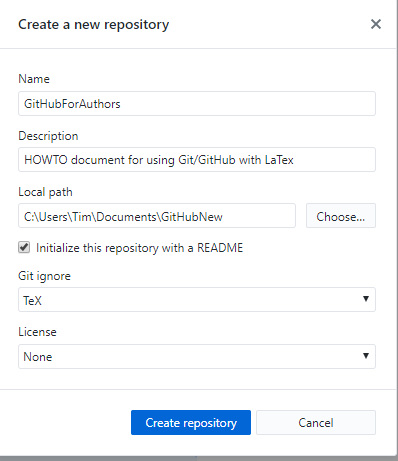
\includegraphics{NewRepo}
\caption{Dialogue to create a new repo.}
\label{newrepo}
\end{figure}

\begin{figure}
\centering
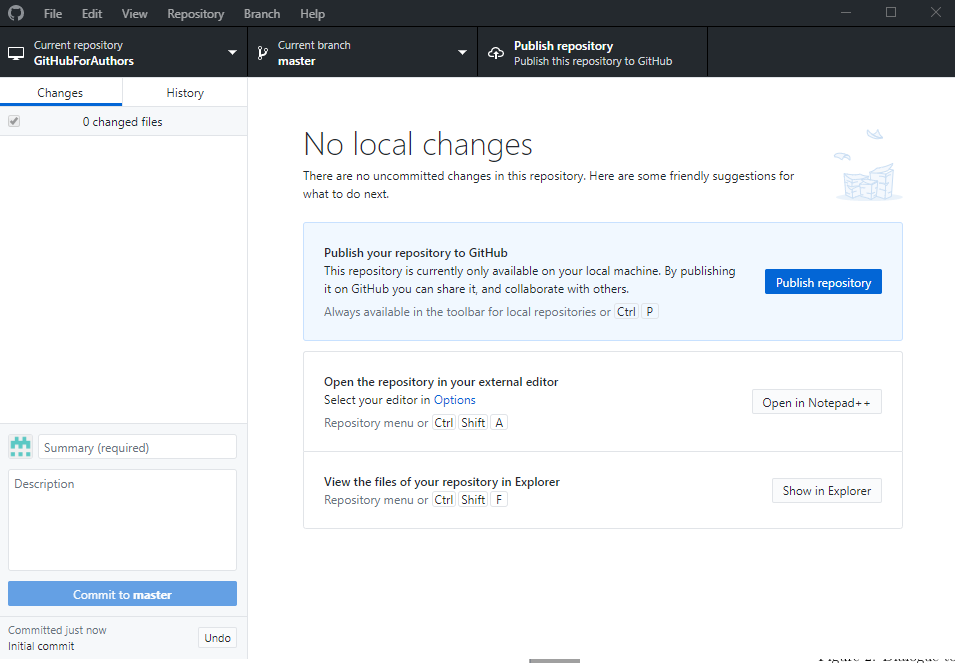
\includegraphics[width=\linewidth]{NewRepoFirstView}
\caption{Desktop view after creating the repo.}
\label{repofirstview}
\end{figure}

The following steps will set up a repo, initialise it with a tex file, make the initial `commit', build the document and make a second `commit' after the build.
\begin{enumerate}
\item Click the `Create New Repository' option, this will give you a new dialogue -- Figure \ref{newrepo}. Fill in the details as required. Initialising with a README file is not essential but good practice. If you are using LaTex then click the drop down against `GitIgnore' and select `Tex'. Click the `Create repository' button. This will lead you to the next screen -- Figure \ref{repofirstview}.
\item If you look in Windows Explorer you should see a folder with three files and one subfolder -- Figure \ref{repofirstviewexplorer}. The `.git' folder is hidden so may not be visible, but this is where all the information for the repo is stored, including the actual files, although not in a format that allows you to view them. If you open the .gitgnore file, you will see that it lists out a large number of file types that Git will ignore. At this stage there is only one branch in this repo -- called `master' -- and in most cases you will probably only need this one branch. If you click on the `History' tab, you will see that Git has recorded the initial creation of the Git files, this is the initial `commit'.
\item Create a tex file in this folder and edit it. Git will pick up the new file and you should see it in the repo view -- Figure \ref{firstfile}. 
\item Create your first commit. A commit is the process of actually getting Git to create internal file objects and track changes, effectively making a snapshot. The boxes in the lower left of the screen should be filled in, the desktop will fill in the small summary description box (you can overwrite this if you wish), but it's good practice to add more to the description box too. You can still make changes at this stage and Git will display them for you, but until they are committed Git won't be tracking anything you do. Click the `Commit to master' button bottom left.
\item Once the commit is complete, the view will revert essentially to that of Figure \ref{repofirstview}, with no local changes being displayed. If you now edit the tex file, you will see how Git records and displays changes -- Figure \ref{firstchange}. There are a few options as this stage:
\begin{itemize}
\item Continue editing.
\item Do another commit.
\item Discard the changes - if you right click the small yellow circle--in--a--square by the file name, this gives you further options, for example to ignore this file, but the first one is to discard the changes. Note that if you do discard changes, Git will edit the file for you on disk, so make sure that's what you really want to do. 
\end{itemize}
If you go to the History tab you will see how your commit has been recorded -- Figure \ref{commithistory}.
\item Edit the tex file such that it will build, then build the document. This will create the usual plethora of LaTex working files, but Git ignore all of these except for the final output (which we assume is a pdf file) -- see Figure \ref{firstbuild} where we can see that all Git has registered is the new pdf file.
\item Do another commit so that Git records the pdf file. In this case the summary description may not be filled in for you, so that needs to be done before Git will allow you to do the commit. Once the commit completes, you will be back to Figure \ref{repofirstview} again.
\end{enumerate}
If you have got this far, then you have basically learnt how to edit and build LaTex whilst recording your changes with Git. If that is all you want to do, i.e. you don't need to use the cloud facilities of GitHub, then, whilst there are some slightly more advanced features described below, you are essentially done.

\begin{figure}
\centering
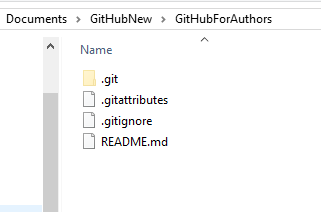
\includegraphics{NewRepoFirstViewExplorer}
\caption{Windows Explorer view after creating the repo.}
\label{repofirstviewexplorer}
\end{figure}


\begin{figure}
\centering
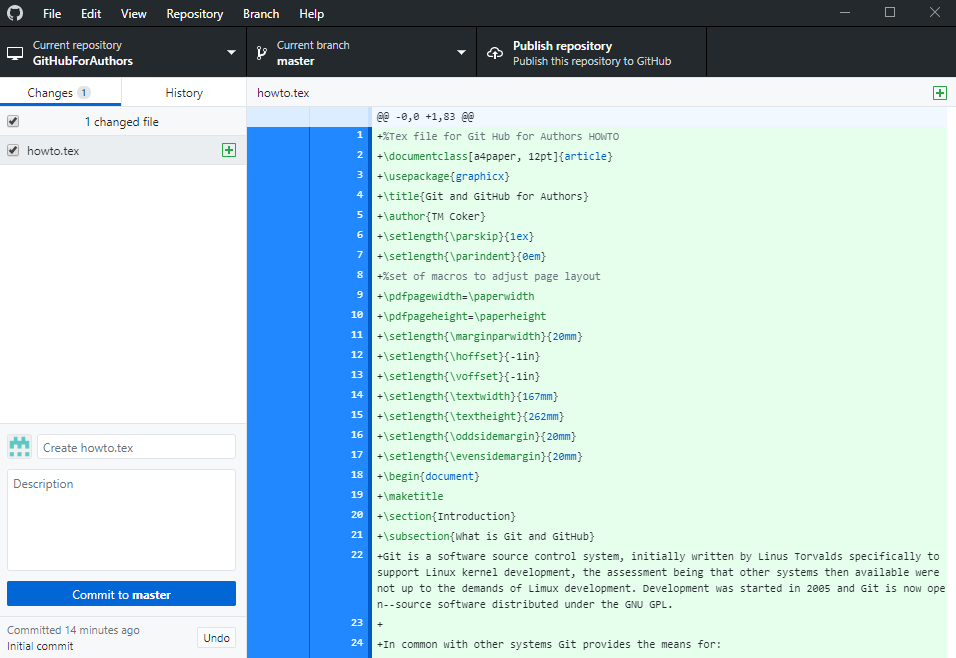
\includegraphics[width=\linewidth]{FirstFile}
\caption{Desktop view after creating the first file.}
\label{firstfile}
\end{figure}

\begin{figure}
\centering
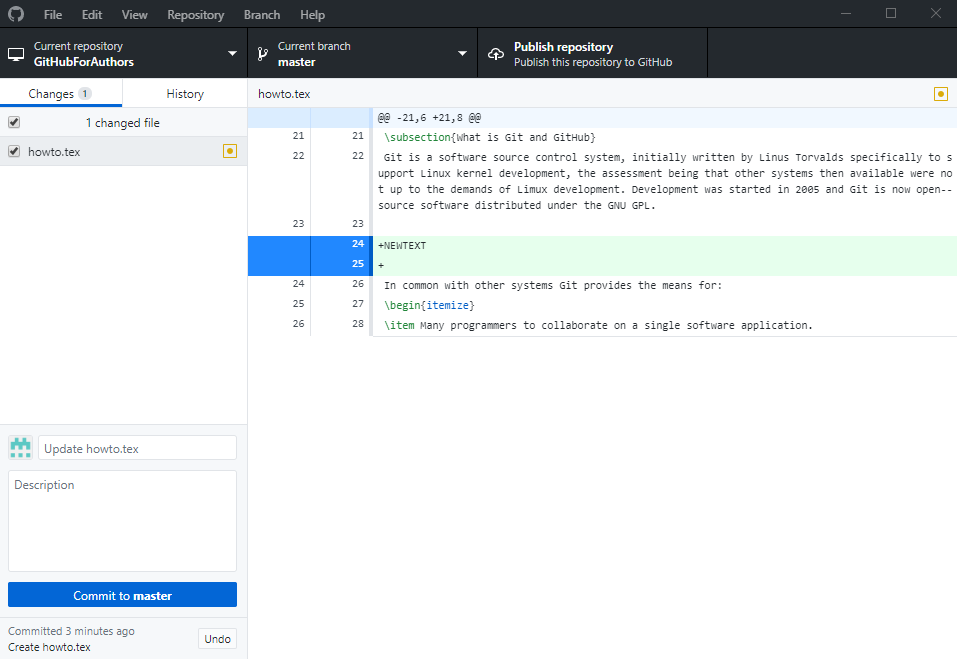
\includegraphics[width=\linewidth]{FirstChange}
\caption{Desktop view after editing a file after a commit.}
\label{firstchange}
\end{figure}

\begin{figure}
\centering
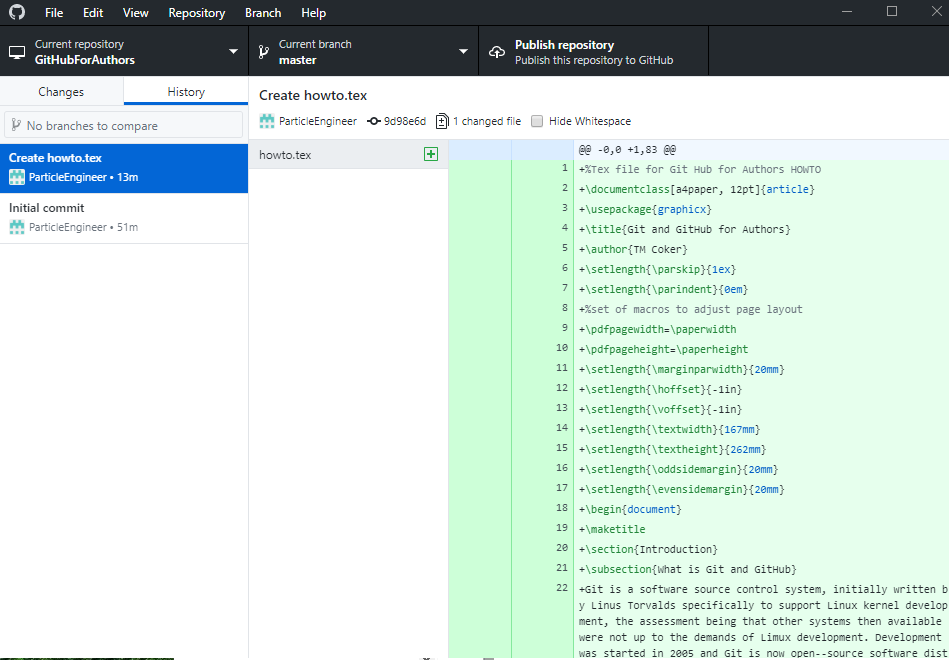
\includegraphics[width=\linewidth]{CommitHistory}
\caption{Desktop view of the History tab.}
\label{commithistory}
\end{figure}

\begin{figure}
\centering
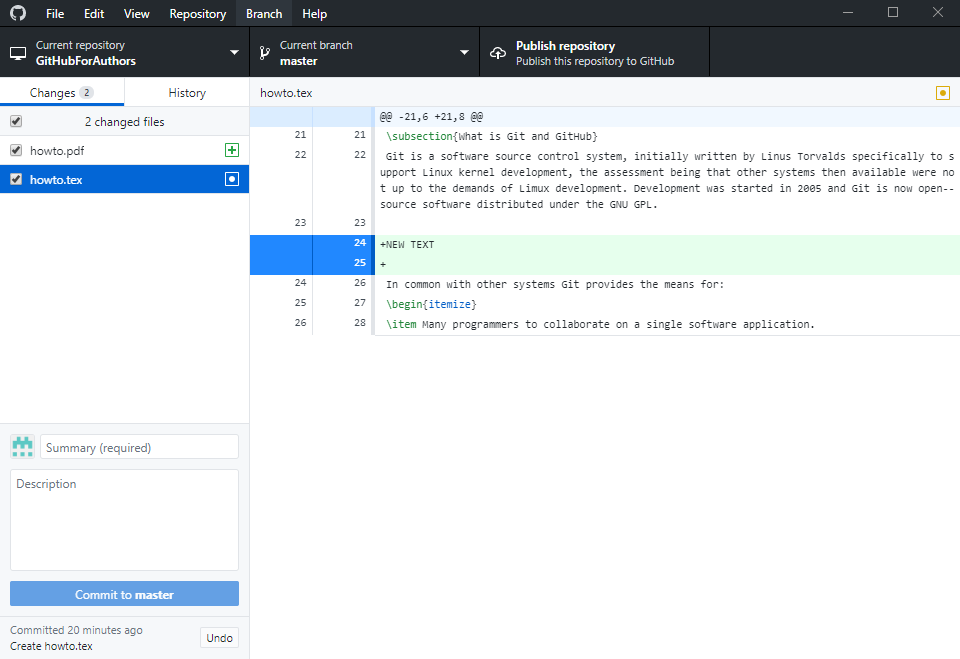
\includegraphics[width=\linewidth]{FirstBuild}
\caption{Desktop view after building the document.}
\label{firstbuild}
\end{figure}

\section{Setting Up and Using GitHub}
You will see in the Desktop that you are being given the option to `publish' your repo to GitHub, there are basically three steps to this -- create an account on GitHub, link it to GitHub Desktop, publish.
\begin{enumerate}
\item Create your GitHub account. This is fairly straight forward, requiring all the usual things you need to create accounts on websites.
\item In the Desktop click the `Publish' button, this will give you a dialogue asking you to log into GitHub. Ignore the Enterprise Server option and sign in. In the following screen you get the option to sign in with the dialogue or through your browser. If you use the dialogue then the process completes more or less automatically, but you should get a message to your GitHub registered email address saying:
\begin{quote}
[GitHub] A first-party GitHub OAuth application has been added to your account.
\end{quote}
This is how GitHub links your deskptop application to your GitHub account. If you instead use the `sign in using your browser' button, this achieves the same end, but with a bit more transparency as to what GitHub is doing.
\item If you now go to your GitHub account in your browser (you may need to log in), you will see that the repo we created above has been published to GitHub, including all the commits we did.
\end{enumerate}
If you now make further changes and commit them, using the same process as above, the next screen is slightly different to Figure \ref{repofirstview}. Here we see that the option now is to `Push' our latest changes to GitHub, see Figure \ref{firstpush}. How often you push chnages to GitHub is up to you, it could be every commit, perhaps if you are making some crucial changes you really don't want to lose, or it could be daily or longer intervals. Note that when you do push, it effectively clones your local repo onto the GitHub remote repo, so \textit{all} your commits, not just the last one, will be pushed.

Other than the advanced topics below, the guide is now more or less complete and you shoudlk be able to manage files with Git and upload them to GitHub.

\begin{figure}
\centering
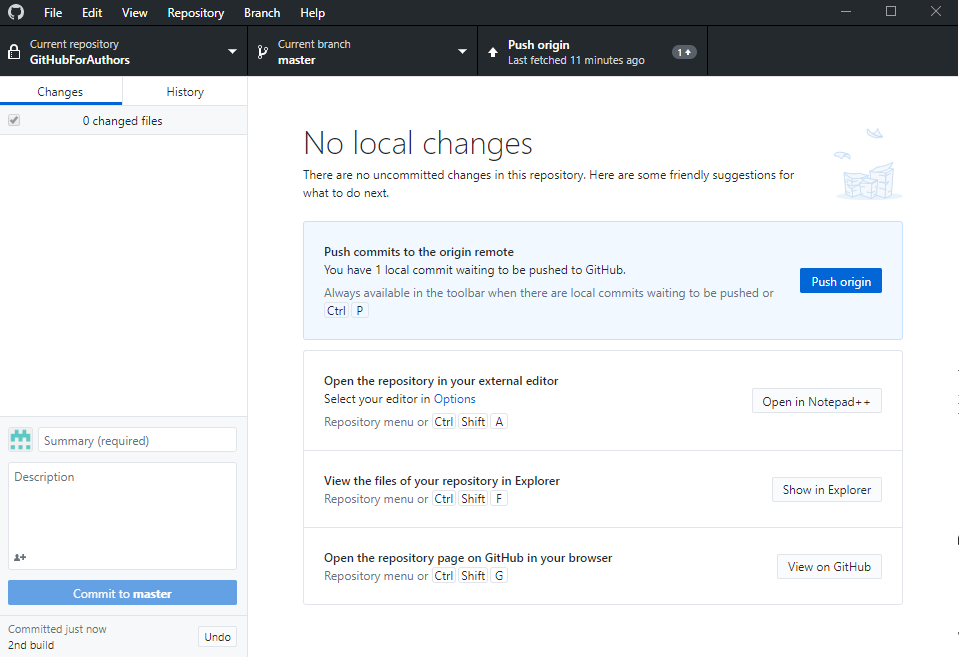
\includegraphics[width=\linewidth]{FirstPush}
\caption{Desktop view after publishing the repo.}
\label{firstpush}
\end{figure}

\section{(Slightly) More Advanced Topics}
\subsection{Working with Branches}
Branches were briefly discussed above; in most cases when writing a document the process is pretty linear and it will probably not be necessary to use branches. However there may be occasions where it becomes appropriate. For example an early draft may be sent out for review, and the easiest way to maintain the source that matches that draft would be to create a branch at that point and carry out further work in the new branch.

Creating a branch is simple enough with the Desktop, just use the menu option `Branch/New Branch...'. Initially the branch is identical to the master, but as you make changes it will, of course, begin to diverge. As the branch is created locally it will not be present in the remote repo on GitHub until it gets published.

Finally a point on how GitHub Desktop works with the file system in Windows. The file folder that the repo is mapped to is effectively a workspace for the \textit{current} branch. This means that if you swap between branches in the same repo, what Git will do is actually delete the files present in the main folder and replace them with the set of files for the branch you're switching to. If there are un--committed changes in the previous branch, you get the option to either `stash' them or take them with you to the next branch. However, if you look in Windows Explorer, it is not apparent which branch is present, you need Git for that. Furthermore, as the switch process involves deleting and creating files, if a file in the previous branch is locked by any other application -- your text editor or MiKTex for example -- then this can cause un--defined behaviour, for example the branch switch fails, or it succeeds but one file that is locked is not deleted, so to Git will appears as a new file in the next branch, and so on. So the message is, take care when switching branches, and in particular make sure that any other application that may be accessing the files is closed.

\subsection{Reverting a Commit}
It may become necessary to revert to a previous commit. This is achieved through the History tab: if you right click in one commit, you get a small dialogue with four options (Figure \ref{revert}), the first of which is to Revert to the selected commit. If you select that option, Git will revert your files back to the state they were in in the selected commit. There are two things to note:

\begin{figure}
\centering
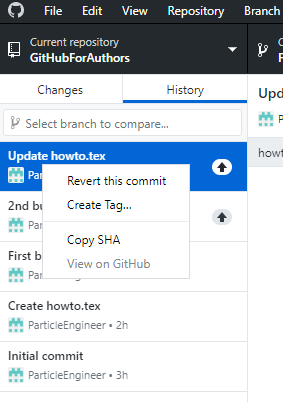
\includegraphics{Revert}
\caption{Reverting to a previous commit.}
\label{revert}
\end{figure}

\begin{itemize}
\item Doing a revert is recorded by Git as if it was any other change, so in principle you can revert the reversion.
\item If you want to revert back more than one commit, you really need to do all the intervening reversions in (reverse) sequence, otherwise Git will start talking about merges and file conflicts.
\end{itemize}
Regarding the last point, if this is really what you want to do, there is a better way (see below), although only if you have pushed changes to GitHub.

\subsection{Tagging}
Tagging (sometimes called labelling) is a standard process where one particular commit is tagged. Typically (when writing software) this is done where a commit aligns with a release, in which case you'd tag the commit with the release version number. Figure \ref{revert} shows the dialogue in the History tag, the second option of which is to create a tag. Any commit can actually be tagged at any time, but it's good practice to tag a commit at the time it is committed. Once tagged, the History tab will show the tagged commit (Figure \ref{tag}).

\begin{figure}
\centering
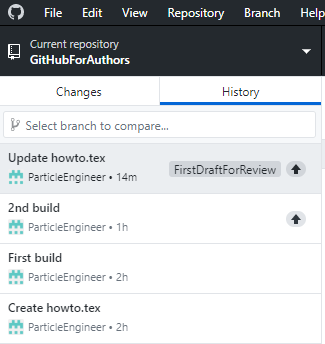
\includegraphics{Tag}
\caption{A tagged commit.}
\label{tag}
\end{figure}

\subsection{Recreating an Older Version}
If it becomes necessary to recreate an older version of a document there are two ways. The first of which would be to revert back to the appropriate commit, but this is complex and perhaps risky and will also load the history with a lot of additional commits that will soon become confusing.

\begin{figure}
\centering
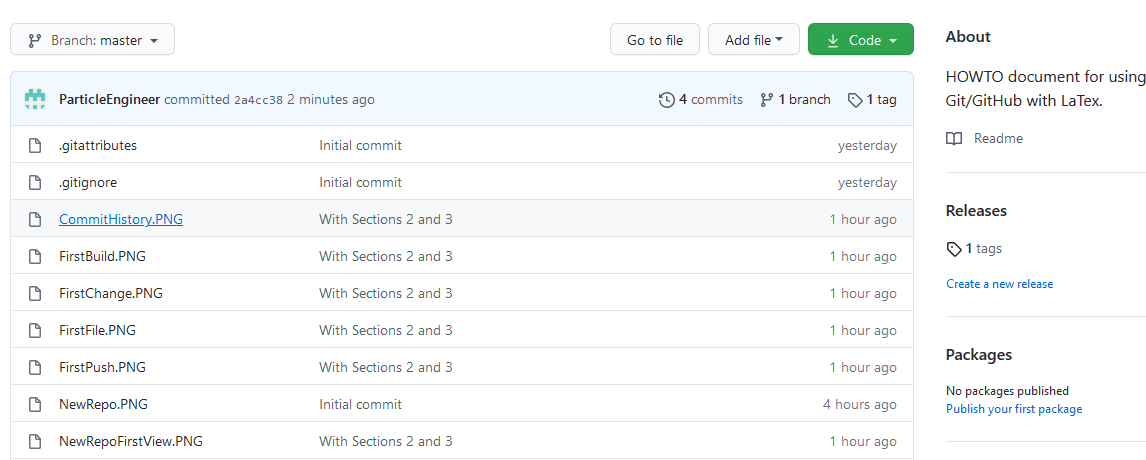
\includegraphics[width=\linewidth]{GHTag}
\caption{Repo on GitHub.}
\label{ghtag}
\end{figure}

The best way to revert back to an older version of a document is to download it from GitHub against a tag. Figure \ref{ghtag} is a view of a repo on GitHub, you can see that this is the master branch and the files displayed are the most current ones. If you click the green Code button you can in fact download a zip of all the files from this commit. If you click on `commits' you will get a page which lists all the commits, and there are options to browse all the files in a particular commit, in which case the Code button will also give you an option to download a zip of files from that particular commit.

\begin{figure}
\centering
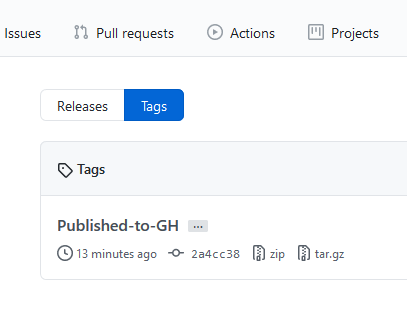
\includegraphics{GHTag2}
\caption{List of tagged commits.}
\label{ghtag2}
\end{figure}

However the easiest option is to tag the commit you are interested in, then you can access that commit directly using the `tags' link under `Releases' (provided, of course, that the tag has been pushed to GitHub). This link will take you to a list of tagged commits and you can download directly from the list, see Figure \ref{ghtag2}. 

Once you have a zip with the tagged files, there are a number of things that could be done. The simplest is just to use the files to re--build the document using MiKTex, without necessarily merging the files back into the repo. However, if you do want this version of your document in Git then there are the following options:
\begin{itemize}
\item Create a new repo. This is the easiest and cleanest solution, but may not always be what you need.
\item Create a new branch, unzip the files into this branch. This will create a branch that matches the tag, but with one commit only.
\item Unzip the files into the current branch and commit.
\end{itemize}


\subsection{Keeping Things Tidy}
One aspect of LaTex is that it does create a lot of additional files. In particular packages such as TikZ-Feynman create a large number of such files. To keep your folder tidy, it often makes sense to put as many of the working files as possible in sub folders. If you do this Git will still find them, and load them into the changes list as long as they are not ignored files.

For a package like TikZ-Feynman, what you end up with is each Feynman diagram being tracked, and often this just clutters the repo without adding much value -- the diagrams can always be re--built from code so storing them on GitHub or in Git has limited value. However you can't simply ignore all pdf files as this will ignore the main file too. In principle you can create a regexp type entry in .gitignore which will cause Git to ignore the figure pdfs, but still see the main output. However the easiest option is to edit .gitignore to ignore the whole folder. This is achieved by adding the following to .gitignore:
\begin{quote}
\# Folder for TikZ-Feynman files

pgf-img/
\end{quote}
Where `pgf-img' is the subfolder that the package uses to create the figures (the comment line isn't strictly necessary of course).

\end{document}